\documentclass[tikz,border=1mm]{standalone}
\usepackage[T1]{fontenc}
\usepackage{lmodern}
\usetikzlibrary{arrows.meta}
\definecolor{navy}{HTML}{17486D}
\definecolor{teal}{HTML}{145B54}
\definecolor{slate}{HTML}{354758}
\begin{document}
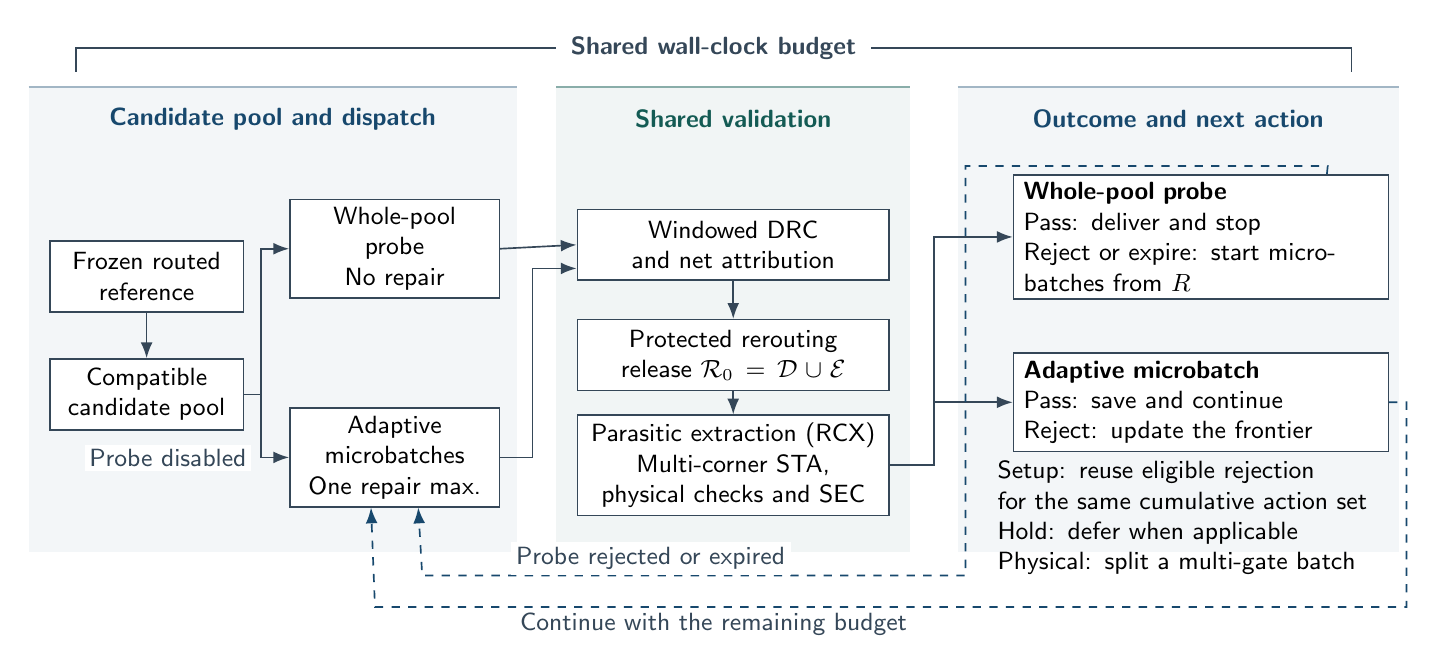
\begin{tikzpicture}[x=1mm,y=1mm,>=Latex, font=\sffamily\small,
  nodebox/.style={draw=slate, line width=.55pt, align=center, fill=white, minimum height=9mm,
                  inner xsep=1.3mm, inner ysep=1.0mm},
  edge/.style={-Latex, line width=.6pt, draw=slate},
  feedback/.style={edge,dashed,draw=navy},
  tag/.style={fill=white,text=slate,align=center,inner sep=.7mm}]
\fill[navy!5] (0,5) rectangle (62,64);
\fill[teal!6] (67,5) rectangle (112,64);
\fill[navy!5] (118,5) rectangle (174,64);
\draw[navy!40,line width=.6pt] (0,64)--(62,64) (118,64)--(174,64);
\draw[teal!50,line width=.6pt] (67,64)--(112,64);
\draw[slate,line width=.55pt] (6,66)--(6,69)--(67,69) (107,69)--(168,69)--(168,66);
\node[fill=white,text=slate,font=\sffamily\bfseries\small] at (87,69) {Shared wall-clock budget};
\node[text=navy,font=\sffamily\bfseries\small] at (31,60) {Candidate pool and dispatch};
\node[text=teal,font=\sffamily\bfseries\small] at (89.5,60) {Shared validation};
\node[text=navy,font=\sffamily\bfseries\small] at (146,60) {Outcome and next action};

\node[nodebox,text width=22mm] (ref) at (15,40) {Frozen routed\\ reference};
\node[nodebox,text width=22mm] (pool) at (15,25) {Compatible\\ candidate pool};
\node[nodebox,text width=24mm] (probe) at (46.5,43.5) {Whole-pool\\probe\\No repair};
\node[nodebox,text width=24mm] (micro) at (46.5,17) {Adaptive\\microbatches\\One repair max.};

\node[nodebox,text width=37mm] (diagnose) at (89.5,44) {Windowed DRC\\ and net attribution};
\node[nodebox,text width=37mm] (route) at (89.5,30) {Protected rerouting\\ release \(\mathcal R_0=\mathcal D\cup\mathcal E\)};
\node[nodebox,text width=37mm] (verify) at (89.5,16) {Parasitic extraction (RCX)\\Multi-corner STA,\\physical checks and SEC};

\node[nodebox,text width=45mm,align=left,anchor=west] (probes) at (125,45)
  {\textbf{Whole-pool probe}\\Pass: deliver and stop\\Reject or expire: start microbatches from \(R\)};
\node[nodebox,text width=45mm,align=left,anchor=west] (micros) at (125,24)
  {\textbf{Adaptive microbatch}\\Pass: save and continue\\Reject: update the frontier};
\node[align=left,text width=49mm,anchor=west,inner sep=0pt] at (123,9.3)
  {Setup: reuse eligible rejection\\for the same cumulative action set\\Hold: defer when applicable\\Physical: split a multi-gate batch};

\draw[edge] (ref)--(pool);
\draw[edge] (pool.east) -- (29.5,25) |- (probe.west);
\draw[edge] (pool.east) -- (29.5,25) |- (micro.west);
\node[tag,anchor=east,font=\sffamily\small,inner sep=.55mm] at (28.3,16.95) {Probe disabled};
\draw[edge] (probe.east) -- (diagnose.west);
\draw[edge] (micro.east) -- (64,17) |- ([yshift=-3mm]diagnose.west);
\draw[edge] (diagnose)--(route);
\draw[edge] (route)--(verify);
\draw[edge] (verify.east) -- (115,16) |- (probes.west);
\draw[edge] (115,16) |- (micros.west);
\draw[feedback] ([xshift=16mm]probes.north) -- (165,54) -- (119,54) --
   (119,2) -- (50,2) -- ([xshift=3mm]micro.south);
\draw[feedback] (micros.east) -- (175,24) -- (175,-2) --
   (44,-2) -- ([xshift=-3mm]micro.south);
\node[tag,anchor=south] at (79,2) {Probe rejected or expired};
\node[tag,anchor=north] at (87,-2) {Continue with the remaining budget};
\end{tikzpicture}
\end{document}